\documentclass{article}

\usepackage[final]{style}
\usepackage[utf8]{inputenc} % allow utf-8 input
\usepackage[T1]{fontenc}    % use 8-bit T1 fonts
\usepackage{hyperref}       % hyperlinks
\usepackage{url}            % simple URL typesetting
\usepackage{booktabs}       % professional-quality tables
\usepackage{amsfonts}       % blackboard math symbols
\usepackage{nicefrac}       % compact symbols for 1/2, etc.
\usepackage{microtype}      % microtypography
\usepackage{verbatim}
\usepackage{graphicx}       % for figures
\usepackage[]{algorithm2e}
\usepackage{amsmath}


\title{Lecture \#19: Introduction to Deep Learning}

\author{
  Robert Yang \\
  Department of Computer Science\\
  Stanford University\\
  Stanford, CA 94305 \\
  \texttt{\{bobyang9\}@cs.stanford.edu} \\
}

\begin{document}

\maketitle

% Done up to Section 2

\section{History of Deep Learning}
Deep Learning is an important technique that can be used for numerous applications including computer vision. How were deep learning methods developed? Historically, the perceptron, the first algorithm that led to deep learning models, was published in a paper by Rosenblatt in 1957. As we will see later, multiple perceptrons could be used together to form a linear classifier. In the 1980s, further improvements on the algorithm such as backpropagation were made and researchers started training the linear classifiers, albeit not very well. In the 1990s, researchers focused on graphical models, and in the 2000s, the support vector machine was very popular. However, in the 2010s, we have revisited the 1980s and the reliance on backpropagation to automatically learn our models. Due to vastly improved computing power (e.g. GPUs) and a large amount of data, the formerly clunky algorithms in the 1980s have become useful and accurate. But to understand today’s advances in deep learning, we must first understand its foundation based in history: the perceptron model, linear classifier, and backpropagation.

\section{The Perceptron}
The structure of the perceptron model is defined by a few key aspects. First, the perceptron takes in some input which we can call $x$. $x$ is a vector, because there can be multiple inputs (e.g. $x_1$, $x_2$, …, $x_n$). Second, the perceptron returns one output which we can call $y$. In the original version of the perceptron, $y$ would be a scalar (one output only). Between the input and the output, the perceptron contains a weighting function that combines the inputs of the perceptron ($x_1$, $x_2$, …, $x_n$) with weights $w$. $w$ is a vector, because there is one weight for each input. Lastly, between the weighting function and the output, there is a sign function, which is usually the following:

\[   \left\{
\begin{array}{ll}
      1 & xw \geq 0 \\
      0 & otherwise \\
\end{array} 
\right. \]

The perceptron algorithm was inspired from biology, but it is not how the brain works! The brain has neurons which gets input through its dendrites, processes that input in the cell body, and then outputs using the axon which might be sent to other neurons. Similarly, the perceptron takes inputs, processes that input, and then outputs the processed result. The weights of the perceptron are analogous to the strength of the connection across the synapses between neurons. However, neurons are probably much more complex than a simple weighting function, which is why the perceptron algorithm is only loosely inspired.

We can gain intuition of the perceptron algorithm by looking at an application related to computer vision. For example, the inputs to the perceptron might represent some sort of image (and we can do this in many different ways, such as using raw pixels, PCA, and BoW, among others). We can convert this input into an output that might signify whether the input is some type of class (e.g. airplane, bird, etc.)

\section{Linear Classifier}

A linear classifier consists of multiple perceptrons put together. For example, you could use a linear classifier to make predictions for multiple classes.

The structure of a linear classifier is similar to the structure of the perceptron. Continuing our computer vision example, we see that the input is the same – a vector $x$ that may perhaps contain information about an image, whether that be a raw pixel representation or some other kind of feature representation. However, the output is now a set of scores (not just one score). For example, you could have a score for the airplane class, for the bird class, etc. We could classify by using the class that has the highest score.

The conversion from input to output in a linear classifier is also defined by the weights $w$, similar to those in a perceptron. $w$ is a 2-D matrix with dimensions (number of classes, number of input elements). We will show why in the example below.

\bigskip

\textbf{Example 1.}

For a certain linear classifier, let there be 10 classes, and let the input be a 32 x 32 x 3 image. Assume that we are using a raw pixel representation. What is the shape of the weight matrix for the classifier?

Answer: First, we must find how many inputs there are. Because we are using a raw pixel representation, the number of inputs will be the number of pixels, which is 32 * 32 * 3 = 3072 inputs. We also know that there are 10 outputs because there are 10 classes (1 output for each class). For each class, we have a set of 3072 weights, and we have 10 sets in total. This will be organized in a (3072, 10) shaped matrix.

\bigskip

As in the example, each class has a set of $n_{input}$ weights, where $n_{input}$ is the dimension of the input vector. You can actually visualize the weights as images:

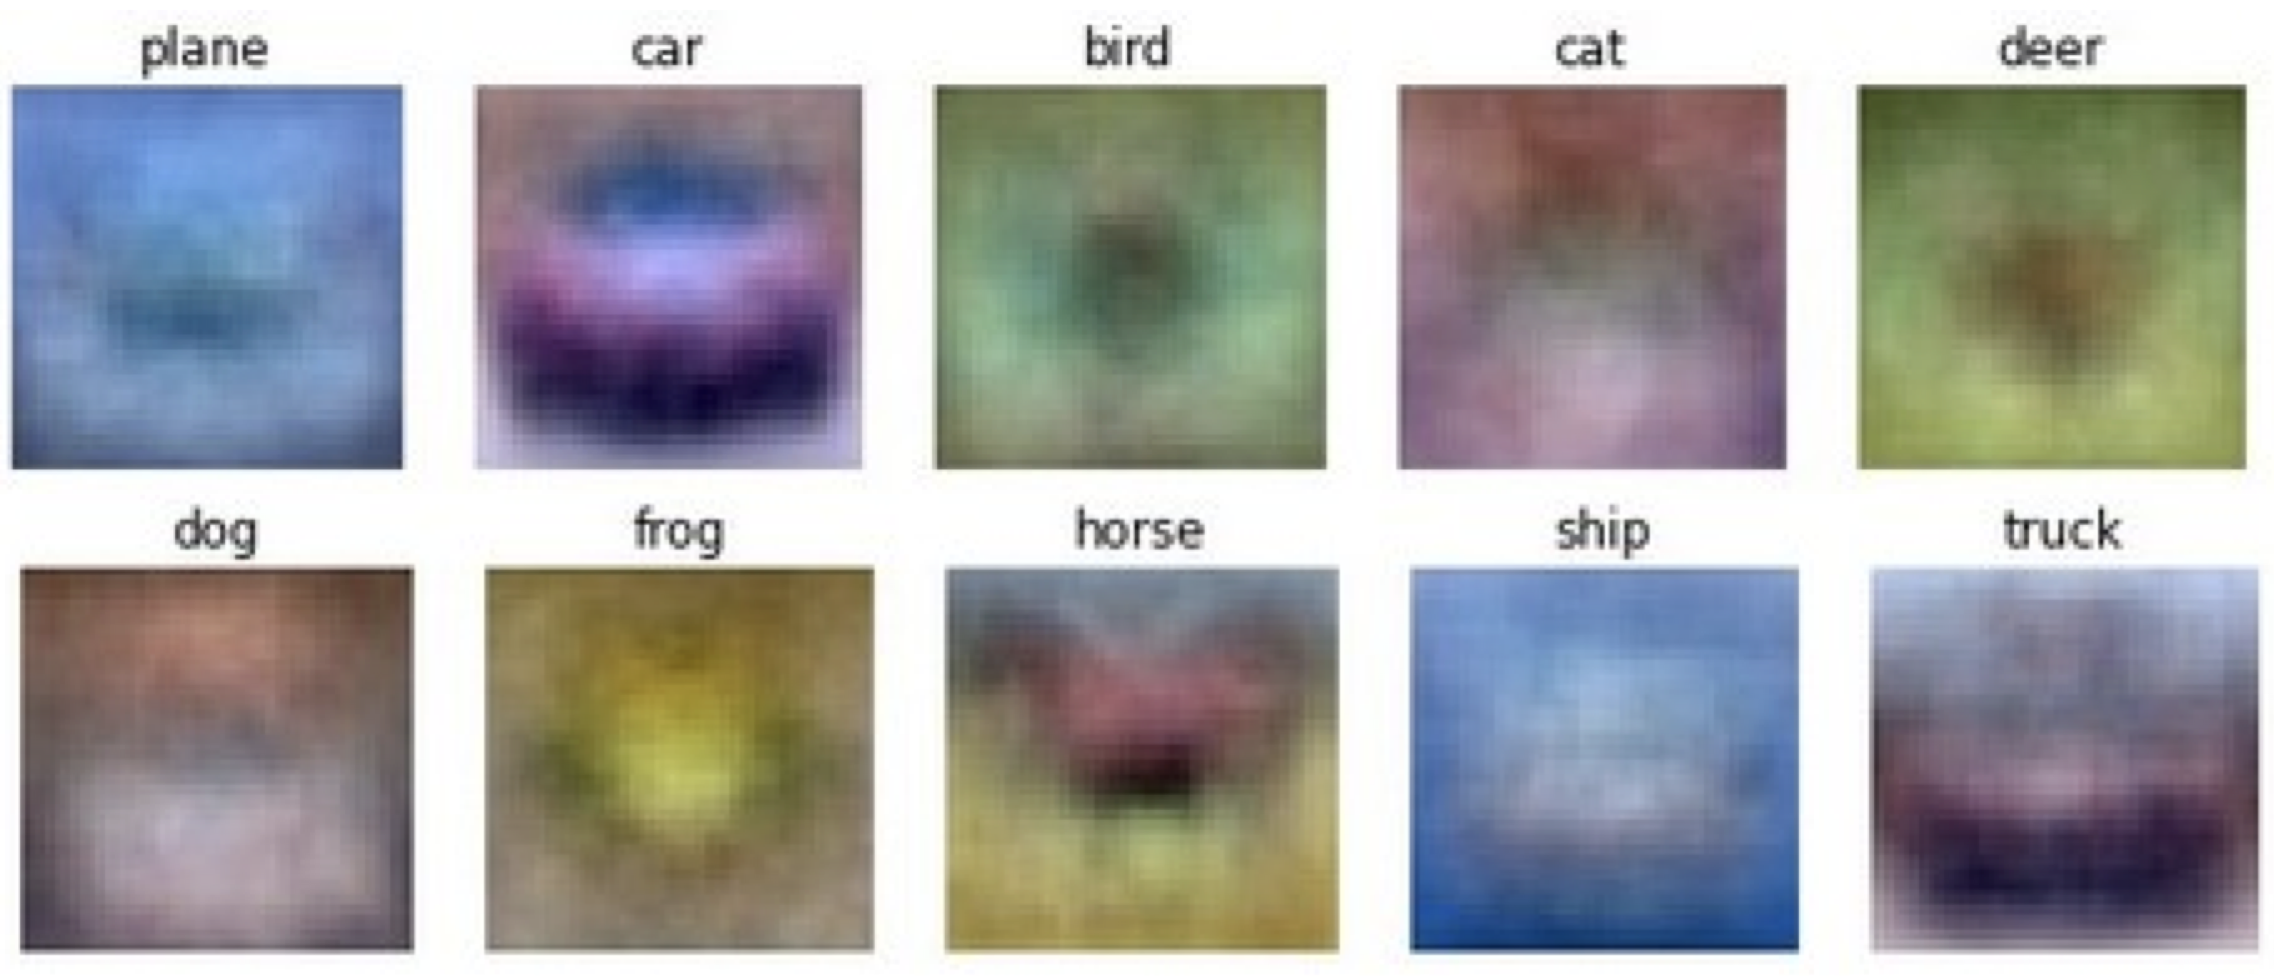
\includegraphics[width=400px]{weights.png}

Sometimes, you also add a bias vector to your results. Intuitively, this helps learn the bias for or against one class in the dataset. For example, if there were more birds in the dataset, you would have a big bias term for the element corresponding to the bird class.

\section{Loss Function}

We need to pick the weights so that they minimize the error our model makes on the dataset. Formally, this is $min_W$ Loss($y$, $\hat{y}$), where $y$ is the true label and $\hat{y}$ is the predicted label.

% The following 2 paragraphs adapted from lecture slide 40.
Given several training examples ${(x_1, y_1), (x_2, y_2), ..., (x_N, y_N)}$ and a perceptron $\hat{y} = wx$, where $x_i$ is an image and $y_i$ is an integer label (0 for dog, 1 for cat, etc.)

A loss function $L_i(y_i, \hat{y_i})$ tells us how good our current classifier is. When the classifier predicts correctly ($y_i$ is close to $\hat{y}$), the loss should be low. When the classifier predicts incorrectly ($y_i$ is far from $\hat{y}$), the loss should be high. We can average the loss over the entire dataset to see how well our model is doing in general.

\subsection{Different Types of Loss Functions}

\textbf{L2} is the squared error loss function. The goal is to minimize the squared difference between the ground truth labels and the predictions. However, the L2 loss is not very robust to outliers. One relatively strange example will increase the loss by a lot.

Formula for L2 loss: $L_i(y_i, \hat{y_i}) = (y_i - \hat{y_i})^2$

\textbf{L1} is a loss function similar to L2 which aims to minimize the absolute value of the difference between the ground truth labels and the predictions. The absolute value is there because you want loss to be positive, and zero loss means that you are able to perfectly classify your dataset.

Formula for L1 loss: $L_i(y_i, \hat{y_i}) = |y_i - \hat{y_i}|$

\textbf{Zero-One} is a loss function that only measures if the predictions are correct or incorrect, and does not measure how correct or incorrect the predictions are. If the model makes an error, then the loss is 1, and if the model does not make an error, then the loss is 0. This loss function has a few weaknesses in that models using this loss function takes longer to train (it is less informative on the correctness of the predictions).

Formula for Zero-One loss: $L_i(y_i, \hat{y_i}) = 1||y_i \neq \hat{y_i}||$

\textbf{Hinge} is another loss function that grows bigger when the difference between the prediction and the ground truth increases.

Formula for Hinge loss: $L_i(y_i, \hat{y_i}) = max(0, 1-y_i\hat{y_i})$

\section{The KL Divergence Loss Function and the Softmax Linear Classifier}

Sometimes we want the model to output probabilities instead of scores because we can visualize probabilities better. We need to convert the vector of scores into a probability distribution.

There are no limits to the output space for the scores of the linear classifier model, which mean that values might appear which do not signify probabilities (values greater than 1 or less than 0). Softmax is a method to convert the output into probability ranges [0, 1]. It does so by taking the exponential of the outputs and then normalizing them, as you will see below in the formula. 

$Prob[f(x_i, W) == k] = \frac{e^{\hat{y}_k}}{\sum_{j}e^{\hat{y}_j}}$

The KL divergence allows you to calculate the distance between two probability distributions. First, we can define $P(y)$ as the ground truth distribution, and $Q(y)$ as the model’s output score distribution (the predictions). KL divergence is defined as the following:

$D_{KL} = \sum_{y}^{} P(y)log\frac{P(y)}{Q(y)}$

Usually, $P(y)$ is probability 1 for one class and 0 for all other classes. In such cases, since $P(y)$ is 0 for all the other classes, [LaTeX from slide 46] can be rewritten as $log (\frac{1}{Q(y)})$, which can be rewritten as $-log(Q(y))$, where $y$ is the class with probability 1 in $P(y)$. 

Notice that softmax and KL divergence work together very well because the exponent and ln will cancel out. Furthermore, inputting the probabilities given by softmax into KL divergence gives a loss from 0 to infinity, which is a good range.

\bigskip

$\textbf{Example 2.}$

Let $C$ be the number of classes in the classifier. In the scenario where the classifier outputs the same result for all the classes, and that softmax is used to normalize output, what would be the KL Divergence loss?

Answer: If the classifier outputs the same result for all the classes, then each class will have a probability of $\frac{1}{C}$ after softmax. We know that the KL divergence loss would be $-log(Q(y))$, and we know that Q(y) is $\frac{1}{C}$ because no matter which of the classes has a 1 in the ground truth, the prediction would be $\frac{1}{C}$. Thus, we would find that the KL divergence loss would be $-log(\frac{1}{C})$, which is $log(C)$.

\bigskip

A summary:

\textbf{Softmax} allows us to convert scores into probabilities.

\textbf{KL Divergence} allows us to calculate the distance between the predicted probabilities and the ground truth.


\section{Gradient Descent}

Gradient Descent is a technique used to find optimal weights that minimize the loss. 

\subsection{Intuition of Gradient Descent}

In Gradient Descent, you iterate through the following loop:

1. You first compute the derivative of the loss with respect to the weights, and with this, you would know which direction to move the weights in order to lower the loss.

2. You would move toward that direction by updating the weights.

You would repeat the two steps until you get to a local minima. In this way, the gradient descent algorithm will slowly decrease the loss.

\subsection{Theory}

We can calculate what the gradient looks like given our loss function. First, we have a training data point (x, y), and we are using the linear classifier where $\hat{y} = wx$. Let us define k as the class which is correct. We know that the loss is -log(softmax($\hat{y}(k)$)), where $\hat{y}(k)$ is the score given to the correct class by the linear classifier.

Evaluating that expression, we get that Loss = $L(\hat{y}, y)$ = $-log\frac{e^{\hat{y}_k}}{\sum_{j}e^{\hat{y}_j}}$ = $-\hat{y}_k + log\sum_j e^{\hat{y}_j}$. 

Now that we have our loss function, we need the derivative of the loss function with respect to each weight, $\frac{dL}{dW}$. However, since the loss function is in terms of $\hat{y}$, we will need to use the chain rule:

$\frac{dL}{dW} = \frac{dL}{d\hat{y}} \frac{d\hat{y}}{dW}$.

First, we need to calculate $\frac{dL}{d\hat{y}}$. To do this, we need to consider 2 cases.

Case 1: We are calculating the derivative respect to $\hat{y}$ for the class k. In this case, the derivative of the loss function is

$\frac{dL}{d\hat{y}_k}$ = $\frac{d}{d\hat{y}_k}(-\hat{y}_k) + \frac{d}{d\hat{y}_k}(log\sum_j e^{\hat{y}_j})$

$ = -1 + \frac{e^{\hat{y}_k}}{\sum_j e^{\hat{y}_j}}$.

Case 2: We are calculating the derivative respect to $\hat{y}$ for a class $l$ where $l \neq k$. In this case, the derivative of the loss function is

$\frac{dL}{d\hat{y}_k}$ = $\frac{d}{d\hat{y}_k}(-\hat{y}_k) + \frac{d}{d\hat{y}_k}(log\sum_j e^{\hat{y}_j})$

= $\frac{e^{\hat{y}_l}}{\sum_j e^{\hat{y}_j}}$.

We also know that since $\hat{y} = Wx$, $\frac{d\hat{y}}{dW} = x.$ Thus, we see that $\frac{dL}{dW} = $
$
\begin{bmatrix} 
\frac{e^{\hat{y}_0}}{\sum_j e^{\hat{y}_j}} \\
\frac{e^{\hat{y}_1}}{\sum_j e^{\hat{y}_j}} \\
... \\
-1 + \frac{e^{\hat{y}_k}}{\sum_j e^{\hat{y}_j}} \\
... \\
\frac{e^{\hat{y}_{n-2}}}{\sum_j e^{\hat{y}_j}} \\
\frac{e^{\hat{y}_{n-1}}}{\sum_j e^{\hat{y}_j}}
\end{bmatrix}
$

where $n$ is the number of classes.

\subsection{Pseudocode of Gradient Descent}

Now, we can translate the theory into code. First, we calculate the loss by looping through each data point and averaging the losses of each data point. Then, we calculate the derivative of the loss with respect to each weight, and update each weight.

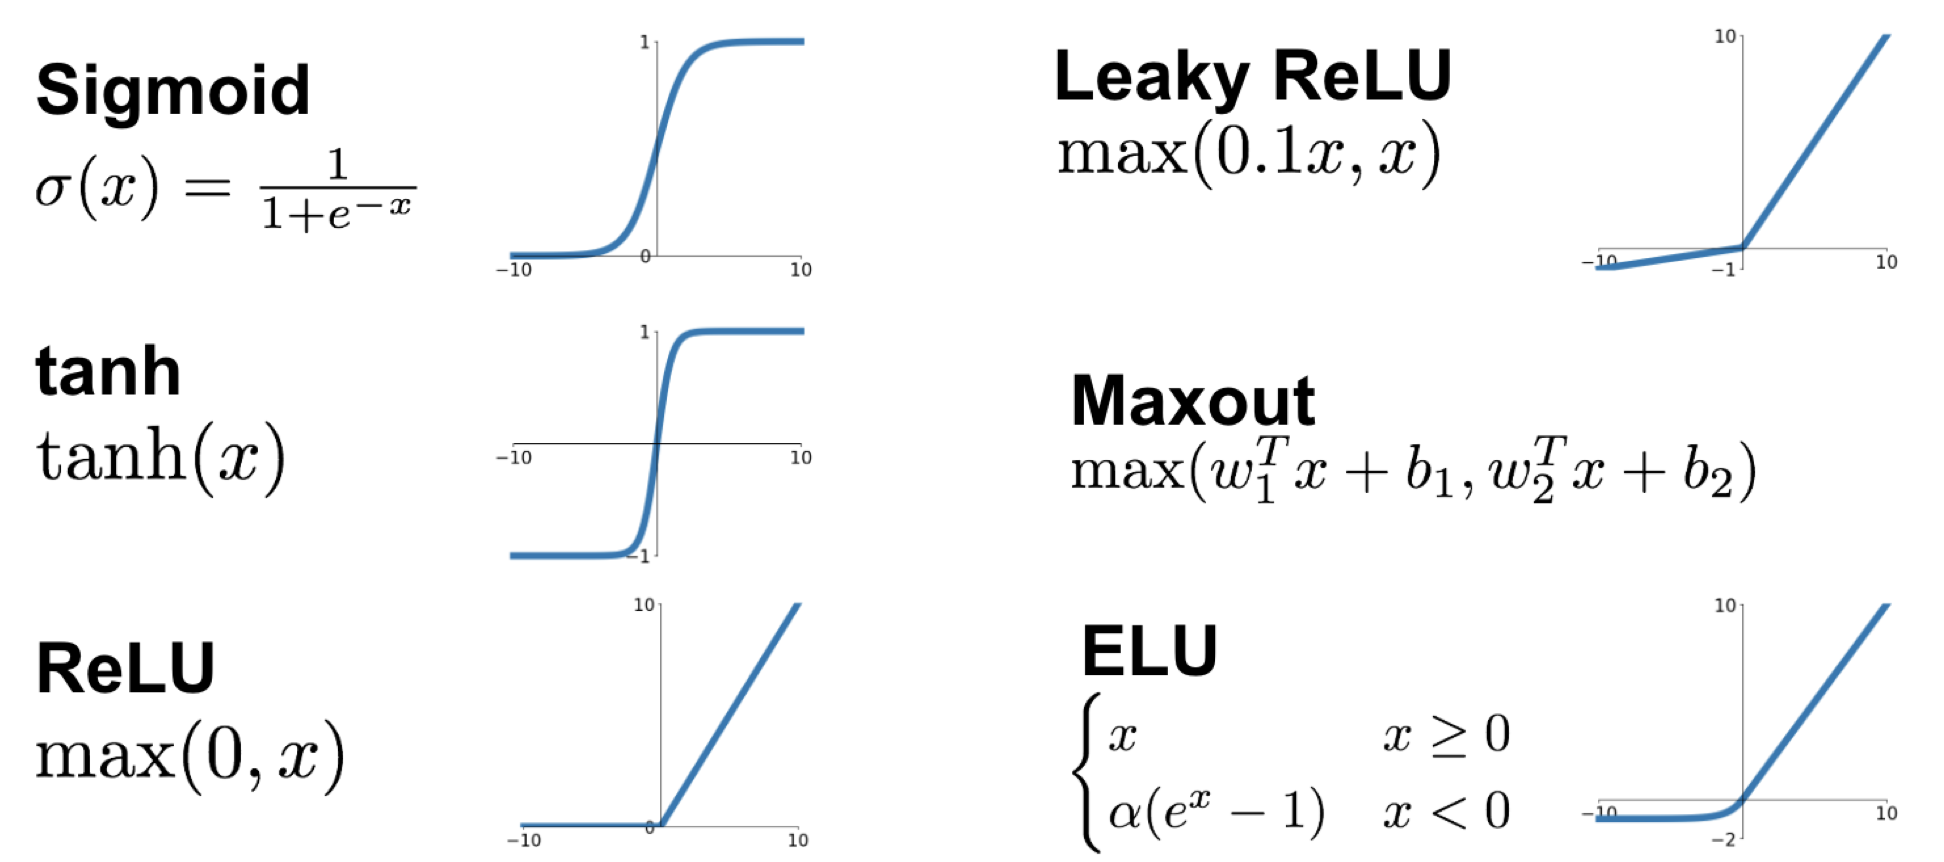
\includegraphics[width=250px]{activation_functions.png}

$\alpha$ is a hyperparameter that represents step size. You can tune this hyperparameter to find the optimal step size. If $\alpha$ is too small, then your algorithm will take a long time (many iterations) to finish, while if $\alpha$ is too big, your algorithm might overshoot the local minima.

% To come next time? 
% \section{Gradient Descent and Backpropagation}
% \section{Neural Networks}
\section{Backpropagation}
Backpropagation is a method to compute the gradients which visualizes the computation as a graph. For example, you would first have a graph to compute the loss:

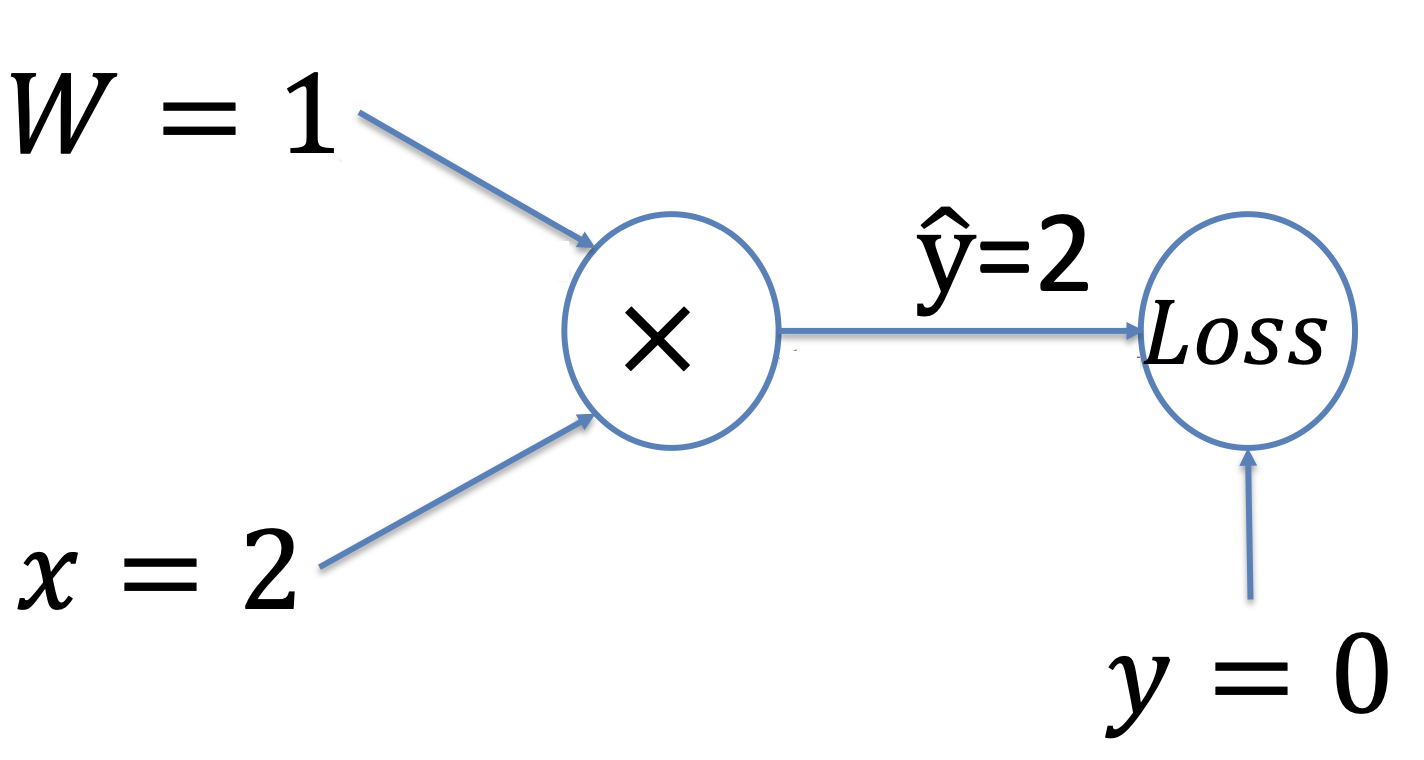
\includegraphics[width=200px]{backprop_pic_2.png}

You would first apply the multiplication operator on W and x to get $\hat{y}$. Afterwards, you would calculate loss from $\hat{y}$ and $y$. This step of going forward to find the loss is called the forward pass.

Afterwards, you go backwards to calculate the gradients:

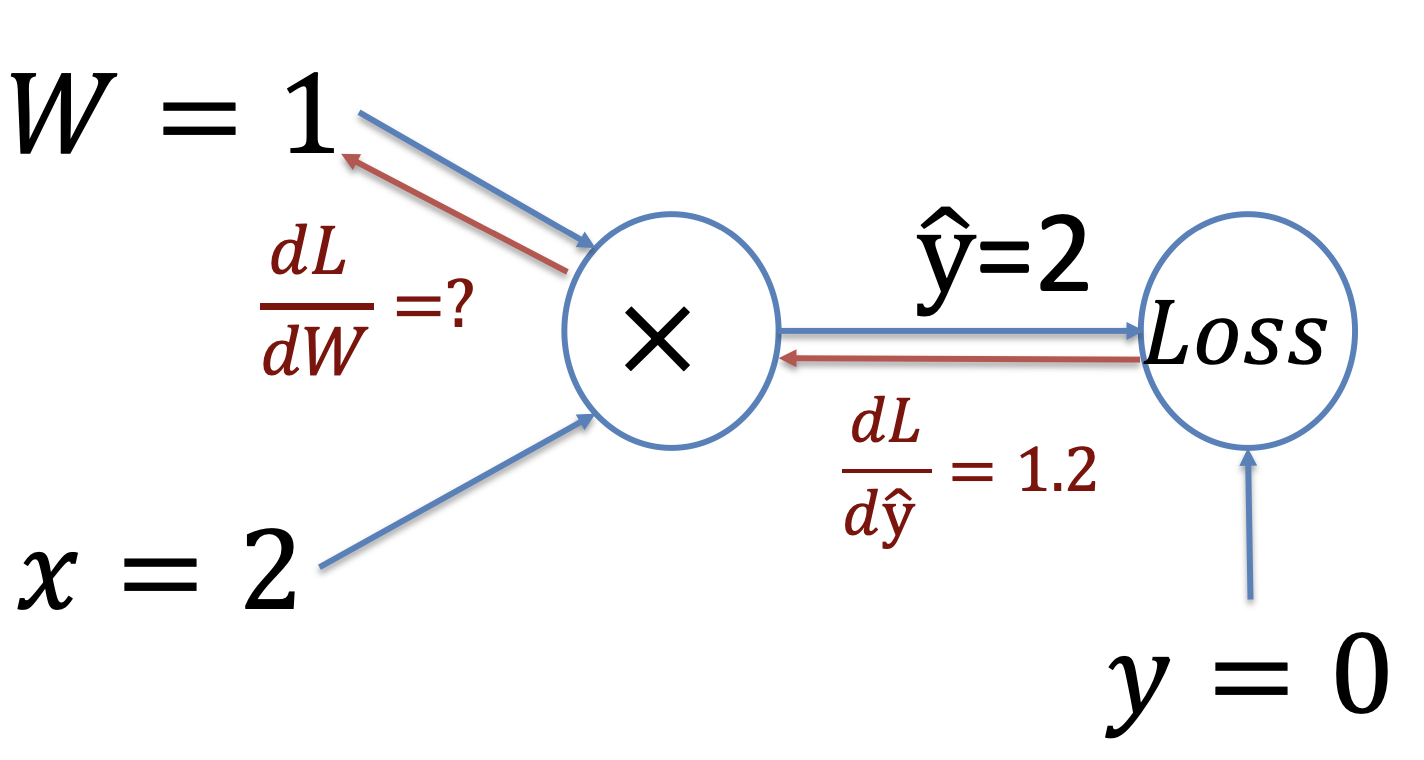
\includegraphics[width=200px]{backprop_pic_1.png}

You first calculate $\frac{dL}{d\hat{y}}$ using the methods described in section 6.2. Then, you can calculate values such as $\frac{dL}{dW}$ by using the chain rule ($\frac{dL}{dW} = \frac{dL}{d\hat{y}} \frac{d\hat{y}}{dW}$). In the above example, because $\hat{y} = Wx$, $\frac{d\hat{y}}{dW} = x = 2$. Thus, $\frac{dL}{dW} = \frac{dL}{d\hat{y}} \frac{d\hat{y}}{dW} = (1.2)(2) = 2.4.$

\section{Neural Networks}

\subsection{Basics of Neural Networks}

We have many ways of producing features for a dataset, including using the raw pixels, injecting positional information using the raw pixels in addition to the (x, y) coordinates, using LDA or PCA to find features that produce the most variance in a supervised or unsupervised manner, or using a set of interesting areas in an image, called a "Bag of Words". If we are using the dataset for classification, we could then use a linear classifier to separate the data. However, sometimes, the data isn't linearly separable, leading the classifier to perform poorly, as in the example below.

Finding good, linearly separable features for use in classification still is a difficult and somewhat finicky task. Namely, we don't know what data we are going to get, and each dataset might require a different feature encoding method to produce the best results possible. However, there is a solution.

The strategy is to design a function to convert features which are not linearly separable into features that are. For example, in the picture below, by applying a transformation to $(r, \theta)$ coordinates, you could now linearly separate the data.

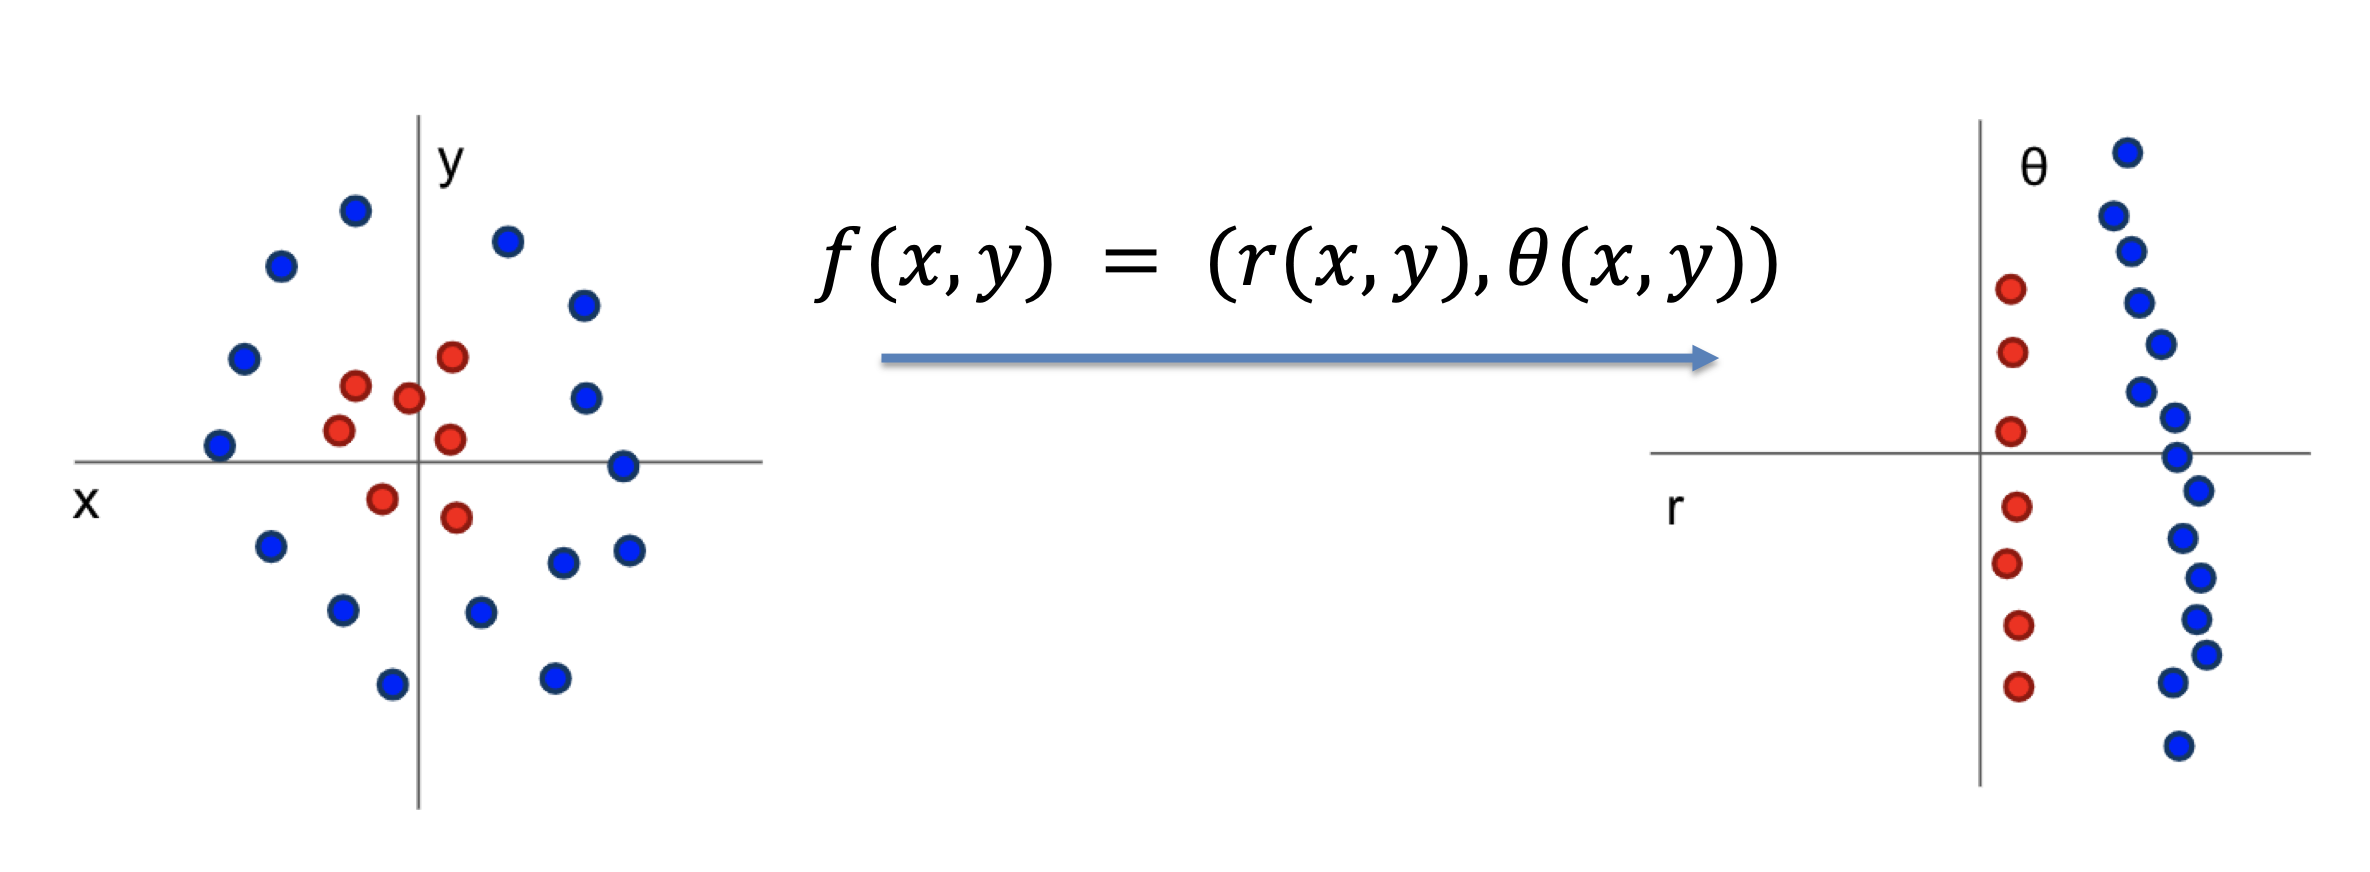
\includegraphics[width=200px]{linearly_separable.png}

In other words, the function will learn what features to input into our linear classifier. The outputs of that function would be the inputs of the linear classifier, which would look something like this:

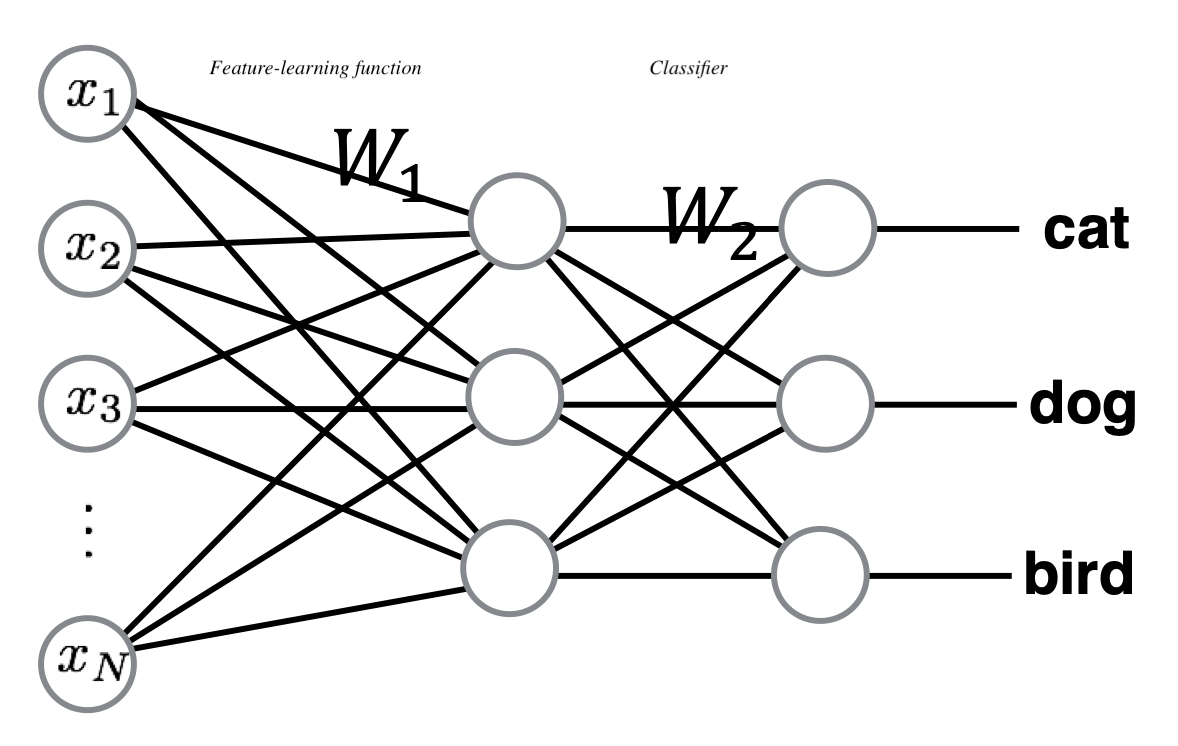
\includegraphics[width=300px]{neural_network.png}

This is a neural network with 2 layers, where the first layer generally works to learn better features and the second layer classifies the better features. Neural networks with $n$ layers have the first $n-1$ layers to learn better features and the last layer, usually a softmax, for the purpose of classification.

For the 2-layer network, we can calculate $\hat{y}$ using the following formula: 

$\hat{y} = W_2max(0, W_1x)$.

Why is the max function necessary? Notice that one property of linear functions like matrix multiplication is that no matter how many of them you apply, the transformation on a whole is linear. Thus, if you got rid of the max function, you would have $\hat{y} = W_2W_1x$, but that would just collapse to $\hat{y}=Wx$ where $W = W_2W_1$.

We can also calculate the shape of the matrices that hold the weights.

\textbf{Example 3.}
Let the shape of $x$, the input, be (3072, 1), let the shape of $y$, the output, be (10, 1), and let the shape of $a$, the hidden units, be (h, 1). What is the shape of $W_1$ and $W_2$?

Answer: Since $a = W_1x$, $W_1$ must be shape (h, 3072) so that $W_1x$ is of shape (h, 1). Also, since $y = W_2a$, $W_2$ must be shape (10, h) so that $W_2a$ is of shape (10, 1).

Note: When designing the structure of the network, we determine the value of $h$, so $h$ is another hyperparameter.

\subsection{Activation Function}
The max function in the formula $\hat{y} = W_2max(0, W_1x)$ for calculating the prediction of a 2-layer neural network is one of many activation functions (also called nonlinearities because they prevent the neural network from collapsing back into one linear combination). Such functions allow models to learn more complex transformations for features. There are many activation functions, as seen below:

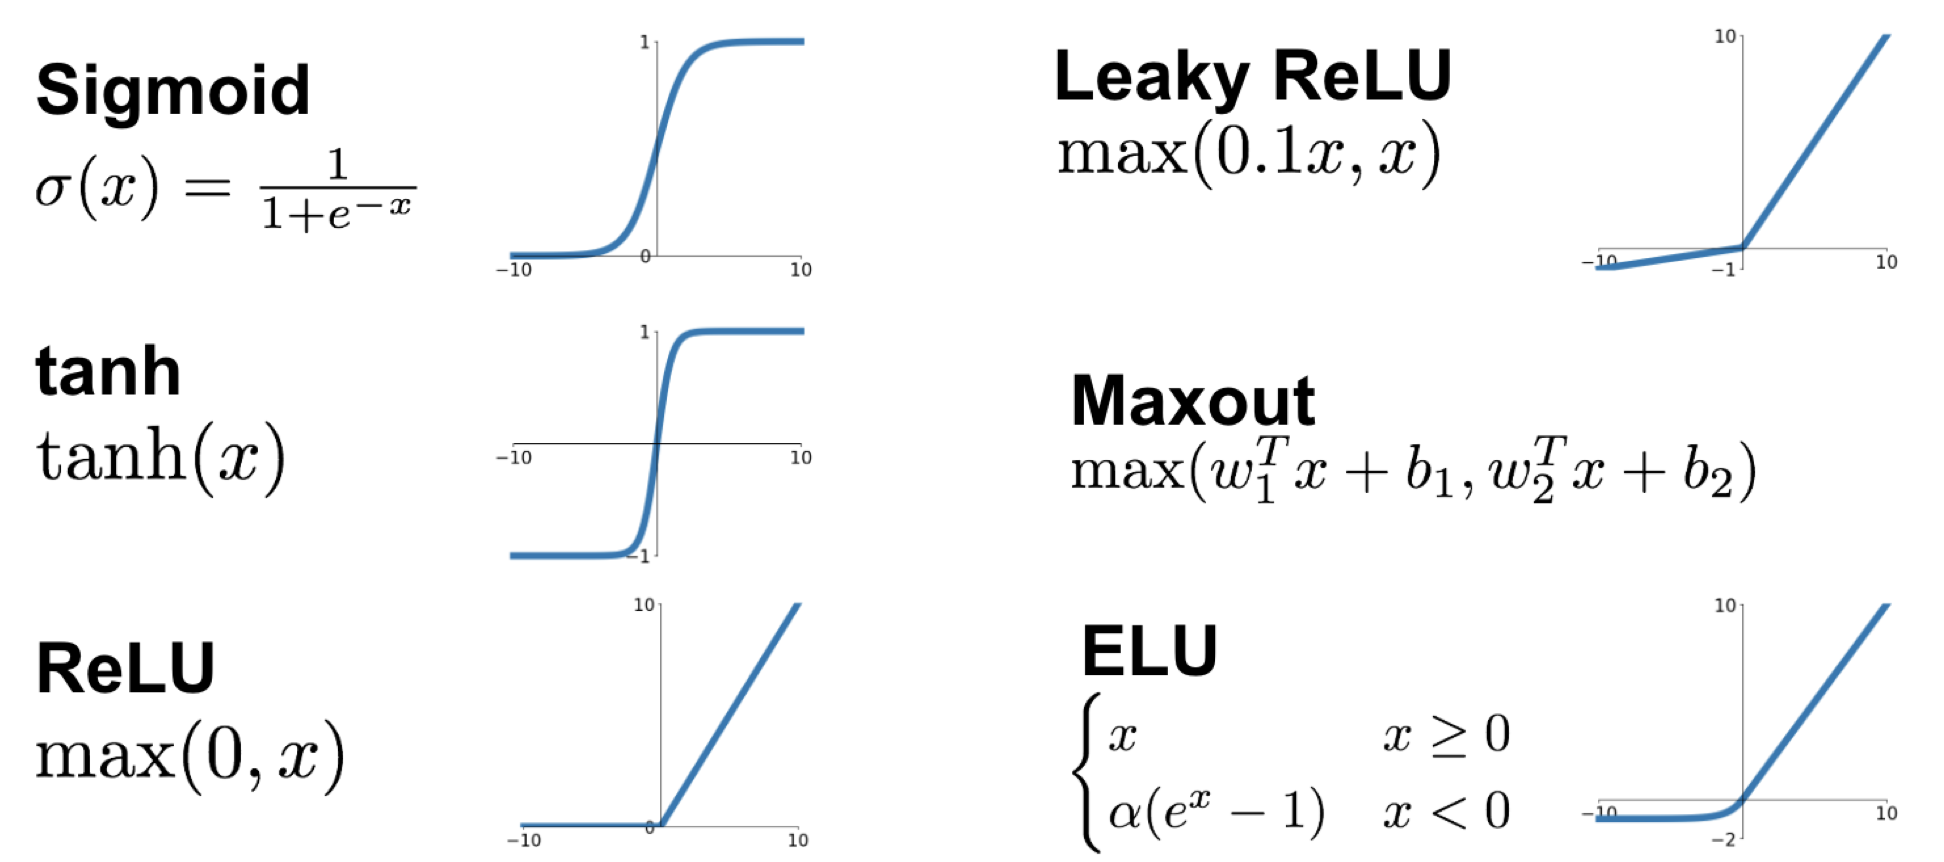
\includegraphics[width=300px]{activation_functions.png}

The sigmoid function is very popular and widely used but one of the slower functions, while tanh is similar to sigmoid in terms of properties but is centered at 0. ReLU (the rectified linear unit) is the function used in most neural networks today because of its double function in providing nonlinearity and regularization, and it is one of the faster functions. Leaky ReLU is an advanced version of ReLU. Finally, Maxout and ELU are less seen but still used in some cases. Choosing the right activation function is another hyperparameter, so try different ones to see which ones work best.

\section{Conclusion}
Understanding the history of deep learning and how the algorithms and models developed will be crucial to understanding how deep learning works. The models of deep learning are made of stacks of linked linear classifiers. Deep learning algorithms evaluate their performance using loss functions. Softmax is still popular in the output of deep learning algorithms. Furthermore, backpropagation and gradient descent (advanced versions of it), which give the model the ability to learn weights, is crucial for performance at increasingly complex tasks in computer vision and elsewhere.


%Deep learning heavily uses all the basic tools such as Linear Classifiers, Loss Functions, Softmax, and Gradient Descent. 

%Deep Learning is a data-intensive approach unlike most of the traditional computer vision algorithms. Thus, it is 
% References
\small
\bibliographystyle{plain}
\bibliography{bibliography}

\bigskip
\end{document}
